\chapter{Splitting Metrics: Entropy and Gini}
\label{chap:splitting_metrics}

\section{The Core Problem: How to Split?}
A Decision Tree makes thousands of cuts. But how does it decide \textit{where} to cut?
Should it split on "Age" or "Income"? Should the threshold be 25 years or 30 years?
\\ To answer this, we need a mathematical way to measure the quality of a split. The goal is to maximize \textbf{Purity}.

\begin{definition}
\textbf{Purity}: A node is "Pure" if it contains samples from only one class (e.g., 100\% Cats). It is "Impure" if it is a mix (e.g., 50\% Cats, 50\% Dogs).
\end{definition}

\section{Entropy (Measure of Surprise)}
Entropy is a concept borrowed from Physics (Thermodynamics) and Information Theory.
\begin{definition}
\textbf{Entropy ($H$)}: A measure of randomness or disorder in a set of data. In Machine Learning, it measures impurity.
\end{definition}

\begin{itemize}
    \item **High Entropy**: High disorder (e.g., A coin flip is 50/50. You are maximally "Surprised" by the outcome).
    \item **Low Entropy**: Low disorder (e.g., An unfair coin that is Heads 99\% of the time. You are not surprised).
\end{itemize}

\subsection{Mathematical Formula}
For a binary classification problem ($p_+$ is probability of Positive, $p_-$ is probability of Negative):
\begin{equation}
    H(S) = - p_+ \log_2(p_+) - p_- \log_2(p_-)
\end{equation}

\subsection{Example Calculation}
Imagine a node with 5 animals: \textbf{2 Cats, 3 Dogs}.
\begin{enumerate}
    \item Probability of Cat ($p_+$) = $2/5 = 0.4$
    \item Probability of Dog ($p_-$) = $3/5 = 0.6$
    \item Calculate Entropy:
\end{enumerate}
$$ H = - [ (0.4 \log_2 0.4) + (0.6 \log_2 0.6) ] $$
$$ \log_2(0.4) \approx -1.32, \quad \log_2(0.6) \approx -0.73 $$
$$ H = - [ (0.4 \times -1.32) + (0.6 \times -0.73) ] $$
$$ H = - [ -0.528 - 0.438 ] = - [-0.966] \approx \mathbf{0.97} $$
\textbf{Conclusion}: $0.97$ is very close to 1. This node is highly impure.

\section{Information Gain}
Identifying impurity is not enough. We want to \textit{reduce} it.
\begin{definition}
\textbf{Information Gain}: The reduction in Entropy after splitting a node on a particular attribute.
\end{definition}
\begin{equation}
    \text{Gain} = H(\text{Parent}) - \sum \frac{N_{\text{child}}}{N_{\text{parent}}} H(\text{Child})
\end{equation}
The algorithm calculates the Information Gain for every possible split and chooses the one with the \textbf{Highest Gain}.

\section{Gini Impurity}
While Entropy is conceptually beautiful, calculating Logarithms ($\log_2$) is computationally expensive for computers.
Most modern libraries (like Scikit-Learn's CART) use \textbf{Gini Impurity} by default.

\begin{definition}
\textbf{Gini Impurity}: A measure of how often a randomly chosen element from the set would be incorrectly labeled.
\end{definition}
\begin{equation}
    \text{Gini} = 1 - \sum_{i=1}^{K} p_i^2
\end{equation}

\textbf{Gini vs Entropy}:
\begin{itemize}
    \item \textbf{Gini}: Max value is 0.5. Computationally faster (squaring is easy).
    \item \textbf{Entropy}: Max value is 1.0. Slower.
    \item \textit{Practical Note}: In 99\% of cases, they yield the same tree. Stick to Gini for speed.
\end{itemize}

\begin{figure}[htbp]
\centering
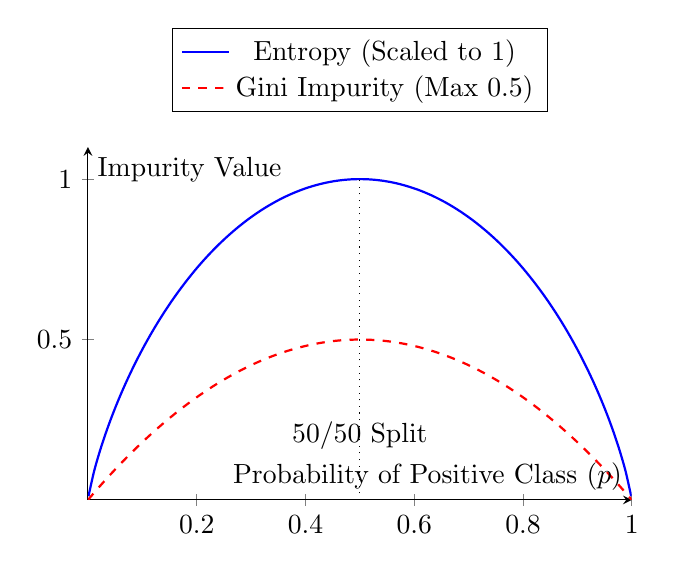
\begin{tikzpicture}
    \begin{axis}[
        xlabel={Probability of Positive Class ($p$)},
        ylabel={Impurity Value},
        xmin=0, xmax=1,
        ymin=0, ymax=1.1,
        axis lines=middle,
        width=0.7\textwidth,
        height=0.5\textwidth,
        legend style={at={(0.5,1.1)},anchor=south}
    ]
    % Entropy Curve
    \addplot[domain=0.001:0.999, samples=100, smooth, thick, blue] {-x*ln(x)/ln(2) - (1-x)*ln(1-x)/ln(2)};
    \addlegendentry{Entropy (Scaled to 1)}
    
    % Gini Curve (Scaled to match height roughly for comparison? No, plot actual Gini)
    \addplot[domain=0:1, samples=100, smooth, thick, red, dashed] {1 - (x^2 + (1-x)^2)};
    \addlegendentry{Gini Impurity (Max 0.5)}
    
    \draw[dotted] (axis cs:0.5, 0) -- (axis cs:0.5, 1);
    \node at (axis cs:0.5, 0.2) {50/50 Split};
    \end{axis}
\end{tikzpicture}
\caption{Comparison of Entropy and Gini. Both are maximized at $p=0.5$ (Maximum uncertainty).}
\label{fig:entropy_gini}
\end{figure}

\section{HOTS: Interview Questions}
\textbf{Q1: What is the difference between Entropy and Gini Impurity?}
\begin{itemize}
    \item Entropy uses logarithms; Gini uses simple squaring.
    \item Entropy ranges from 0 to 1; Gini ranges from 0 to 0.5 (for binary).
    \item In practice, they usually produce identical trees.
\end{itemize}

\textbf{Q2: Why is Information Gain sometimes biased towards features with many values?}
\begin{itemize}
    \item If a feature has many unique values (e.g., ``Customer ID'' with 1000 values), splitting on it creates very ``pure'' leaves (each leaf has one customer). 
    \item This leads to high Information Gain but severe overfitting.
    \item Solution: Use Gain Ratio (C4.5) or Gini (CART).
\end{itemize}

% ========================================
% SECTION: QUICK REFERENCE
% ========================================
\section{Quick Reference Card}

\begin{center}
\fbox{\parbox{0.9\textwidth}{
\textbf{SPLITTING METRICS - CHEAT SHEET}
\vspace{0.3cm}

\textbf{Entropy} (Information Theory):
$$H = -\sum_{i=1}^{K} p_i \log_2(p_i)$$
Range: 0 (pure) to $\log_2(K)$ (max uncertainty)

\textbf{Gini Impurity} (Probability-based):
$$Gini = 1 - \sum_{i=1}^{K} p_i^2$$
Range: 0 (pure) to $1 - 1/K$ (For binary: max 0.5)

\textbf{Information Gain}:
$$IG = H_{parent} - \sum \frac{n_{child}}{n_{parent}} H_{child}$$

\textbf{Comparison}:
\begin{center}
\begin{tabular}{|l|l|}
\hline
\textbf{Entropy} & Uses log, slightly slower \\ \hline
\textbf{Gini} & Faster, default in sklearn \\ \hline
\textbf{Trees?} & Usually identical \\ \hline
\end{tabular}
\end{center}

\textbf{Interview Gold}:
\begin{itemize}
    \item Pure node = Entropy/Gini = 0
    \item 50/50 split = maximum impurity
    \item IG bias: use Gain Ratio for many-valued features
\end{itemize}
}}
